\documentclass[12pt]{article}
\usepackage[utf8]{inputenc}
\usepackage{lineno}
\usepackage{authblk}
\usepackage[margin=1in]{geometry}
\usepackage{xparse}
\usepackage{xpunctuate}
\usepackage{xspace}
\usepackage{graphicx}
\usepackage{wrapfig}
\usepackage[hidelinks]{hyperref}
\usepackage[all]{hypcap}
\usepackage{amsmath}
\usepackage{cleveref}
\usepackage{placeins}
\usepackage{flafter}
\usepackage{floatrow}
\usepackage{subcaption}
\usepackage{minted} 
\setminted[python]{breaklines}
\usepackage{caption}
\usepackage{float}
\usepackage{csvsimple}
\usepackage{booktabs}
\usepackage{siunitx}
\usepackage{natbib}

% local definitions
\newcommand{\msprime}[0]{\texttt{msprime}\xspace}
\newcommand{\tskit}[0]{\texttt{tskit}\xspace}
\newcommand{\slim}[0]{\texttt{SLiM}\xspace}
\newcommand{\pyslim}[0]{\texttt{pyslim}\xspace}
\newcommand{\stdpopsim}[0]{\texttt{stdpopsim}\xspace}
\newcommand{\allel}[0]{\texttt{scikit-allel}\xspace}
\newcommand*{\eg}{e.g.\xcomma}
\newcommand*{\ie}{i.e.\xcomma}
\newcommand{\comment}[1]{\textit{\color{green} #1}}
\newcommand{\p}[1]{\texttt{p#1}}

% syntax highlighting
\usepackage{listings}
\usepackage{xcolor}

% see listings documentation
\lstdefinelanguage{slim}{
    % Eidos language keywords from 
    % https://github.com/MesserLab/SLiM/blob/4bcc36a02aeacdc9ee808e38d62836f854246502/eidos/eidos_token.h#L90
    morekeywords=[1]{if,else,do,while,for,in,next,break,return,function},
    % SLiM callback keywords from
    % https://github.com/MesserLab/SLiM/blob/4bcc36a02aeacdc9ee808e38d62836f854246502/core/slim_eidos_block.cpp#L32
    morekeywords=[2]{first,early,late,initialize,mutationEffect,fitnessEffect,interaction,mateChoice,modifyChild,recombination,mutation,survival,reproduction},
    % Other special SLiM tokens from
    % https://github.com/MesserLab/SLiM/blob/4bcc36a02aeacdc9ee808e38d62836f854246502/QtSLiM/QtSLiMSyntaxHighlighting.cpp#L294
    morekeywords=[3]{sim,community,slimgui,
        p0,p1,p2,p3,p4,p5,p6,p7,p8,p9,p10,p11,p12,p13,p14,p15,p16,p17,p18,p19,p20,p21,p22,p23,p24,p25,
        p26,p27,p28,p29,p30,p31,p32,p33,p34,p35,p36,p37,p38,p39,p40,p41,p42,p43,p44,p45,p46,p47,p48,p49,p50,
        g0,g1,g2,g3,g4,g5,g6,g7,g8,g9,g10,g11,g12,g13,g14,g15,g16,g17,g18,g19,g20,g21,g22,g23,g24,g25,
        g26,g27,g28,g29,g30,g31,g32,g33,g34,g35,g36,g37,g38,g39,g40,g41,g42,g43,g44,g45,g46,g47,g48,g49,g50,
        m0,m1,m2,m3,m4,m5,m6,m7,m8,m9,m10,m11,m12,m13,m14,m15,m16,m17,m18,m19,m20,m21,m22,m23,m24,m25,
        m26,m27,m28,m29,m30,m31,m32,m33,m34,m35,m36,m37,m38,m39,m40,m41,m42,m43,m44,m45,m46,m47,m48,m49,m50,
        s0,s1,s2,s3,s4,s5,s6,s7,s8,s9,s10,s11,s12,s13,s14,s15,s16,s17,s18,s19,s20,s21,s22,s23,s24,s25,
        s26,s27,s28,s29,s30,s31,s32,s33,s34,s35,s36,s37,s38,s39,s40,s41,s42,s43,s44,s45,s46,s47,s48,s49,s50,
        i0,i1,i2,i3,i4,i5,i6,i7,i8,i9,i10,i11,i12,i13,i14,i15,i16,i17,i18,i19,i20,i21,i22,i23,i24,i25,
        i26,i27,i28,i29,i30,i31,i32,i33,i34,i35,i36,i37,i38,i39,i40,i41,i42,i43,i44,i45,i46,i47,i48,i49,i50},
    sensitive=true,
    morecomment=[l]{//},
    morestring=[b]",
}
% colors from 
% https://github.com/MesserLab/SLiM/blob/4bcc36a02aeacdc9ee808e38d62836f854246502/QtSLiM/QtSLiMSyntaxHighlighting.cpp#L139
% numberLiteralFormat.setForeground(inDarkMode ? QColor(115, 145, 255) : QColor(28, 0, 207));
% stringLiteralFormat.setForeground(inDarkMode ? QColor(220, 98, 90) : QColor(196, 26, 22));
% commentFormat.setForeground(inDarkMode ? QColor(90, 210, 90) : QColor(0, 116, 0));
% identifierFormat.setForeground(inDarkMode ? QColor(70, 205, 216) : QColor(63, 110, 116));
% keywordFormat.setForeground(inDarkMode ? QColor(220, 83, 185) : QColor(170, 13, 145));
\definecolor{slimstring}{RGB}{196,26,22}
\definecolor{slimcomment}{RGB}{0,116,0}
\definecolor{slimidentifier}{RGB}{63,110,116}
\definecolor{slimkeyword}{RGB}{170,13,145}
\definecolor{slimstage}{RGB}{0,0,0}
\definecolor{codegray}{RGB}{128,128,128}
% Light beige background for SLiM code (different from Python's gray background)
\definecolor{backcolour}{rgb}{0.95,0.95,0.92}
\lstdefinestyle{slimstyle}{
    language=slim,
    backgroundcolor=\color{backcolour},
    commentstyle=\color{slimcomment},
    keywordstyle=[1]\color{slimkeyword},
    keywordstyle=[2]\color{slimstage},
    keywordstyle=[3]\color{slimidentifier},
    numberstyle=\tiny\color{codegray},
    stringstyle=\color{slimstring},
    basicstyle=\ttfamily\small,
    escapeinside={*@}{@*},
    breakatwhitespace=false,         
    breaklines=true,                 
    captionpos=b,                    
    keepspaces=true,                 
    numbers=left,                    
    numbersep=2pt,                  
    showspaces=false,                
    showstringspaces=false,
    showtabs=false,                  
    tabsize=2
}
\lstset{style=slimstyle}

% Fix for quote encoding issues
% https://tex.stackexchange.com/questions/736299/latex-error-command-textquotedbl-unavailable-in-encoding-ot1
\lstset{upquote=true,basicstyle=\fontencoding{T1}\selectfont}

\definecolor{bg}{rgb}{0.95,0.95,0.98}
\newminted[pycon]{pycon}{bgcolor=bg, linenos=true, tabsize=4}

%\linenumbers

\begin{document}

\title{Bridging forward-in-time and coalescent simulations using pyslim}
\author[1]{Shyamalika Gopalan}
\author[2,3]{Murillo F. Rodrigues}
\author[3,4]{Peter L. Ralph}
%\author[5]{Ben Haller}

\affil[1]{Department of Genetics and Biochemistry and Center for Human Genetics, Clemson University}
\affil[2]{Division of Genetics, Oregon National Primate Center, Oregon Health \& Science University}
\affil[3]{Department of Biology and Institute of Ecology and Evolution, University of Oregon}
\affil[4]{Department of Mathematics, University of Oregon}
%\affil[5]{Department of Computational Biology, Cornell University}

\maketitle

\abstract{
    Ancestral Recombination Graphs (ARGs)
    provide an expressive and compact way to represent genetic variation data generated by simulations
    embedded within its genealogical history,
    and can dramatically speed up simulations.
    The fact that the ARG records genealogical as well as genomic information
    opens up the possibility for a number of new analysis and simulation techniques.
    Here, we aim to introduce the reader to this deep source of information
    as produced by the forwards simulator SLiM.
    SLiM records the ARG using the \emph{tree sequence} format,
    which can be manipulated using the \tskit and \pyslim python packages.
    We first describe the information that SLiM records in the tree sequence,
    then provide several examples that use the tree sequence as a format
    to losslessly pass population states between simulators:
    \emph{recapitation} of a fowards simulation with coalescent simulation;
    initiation of a forwards simulation using the results of a coalescent simulation;
    and parallelization of simulations across branches of a phylogenetic tree.
}
\date{}


\section*{Introduction}
% The importance of simulations in popgen and flavors of simulations
Simulations have become an invaluable tool in population genetics over the past six decades,
allowing researchers to model increasingly complex evolutionary scenarios.
%because of the difficulty in obtaining analytical solutions to complex evolutionary scenarios.
A robust research community has grown around developing computational methods for conducting these
simuations, as well as for representing and analyzing the data that they produce.
Indeed, in prior chapters, two of the most widely used population genetic simulation tools were presented: \slim \citep{haller_slim_2023} and \msprime \citep{baumdicker_efficient_2022}.
% refer to other chapters here?

In this chapter, we present \pyslim, a Python package that facilitates \emph{hybrid simulations},
which are frequently used to combine key features of the two main methods of individual-based population genetic simulation.
These two methods differ primarily in the direction of the simulation
process -- either forward- or backward-in-time. 
The coalescent process models the ancestry of sampled genomes
backward-in-time until they coalesce into their most common recent ancestor. % (MRCA).
This approach is extremely efficient because it only has to simulates the ancestors that directly contributed to the sampled genomes,
thus avoiding the need to represent large swathes of the population pedigree. 
The downside of this approach is its strict assumptions (\eg neutrality, random mating within subpopulations), 
which limit applicability.
On the other hand, forward-in-time simulations start with the ancestral individuals and apply demographic processes rules (\eg reproduction, migration, mutation) over generations.
This affords forward-in-time simulations much more flexibilty,
but at a higher computational cost.
% refer to msprime and SLiM chapters explicitly here?
% The pyslim package and overview of the chapter

Hybrid simulations have recently emerged as a strategy for leveraging the benefits of both forward-in-time and coalescent methods, as well as parallel computing,
to efficiently model highly complex evolutionary scenarios.
Many forward-in-time simulations conducted using \slim, for example, are later modified using the coalescent process to ensure the coalescence of the individuals in the first generation, a process known as \emph{recapitation} \citep{haller_tree-sequence_2019}, which will be discussed in more detail later in this chapter.
These are regularly used in various ways in the literature:
for instance, \stdpopsim, a Python package that stores a large number of published population genetic models,
uses recapitation ensure the coalescence of the individuals in the first generation of the forward-in-time simulation \citep{adrion_community-maintained_2020,elise_expanding_nodate,gower_accessible_2025}.
Similarly, in complex spatial forward-in-time simulations, a coalescent component is almost always used to generate initial diversity,
because it can reduce significantly the computational burden of these simulations \citep{battey_space_2020,petr_slendr_2023}.
\citet{rodrigues_shared_2024} performed whole-chromosome simulations of 10 million yars of the entire great apes history,
which would not have been possible without hybrid simulation techniques.

% something here to motivate the pathogen evolution scenario we present?

A key innovation that has enabled the rise of hybrid simulations is the concept of the Ancestral Recombination Graph (ARG), reviewed in \citet{wong_general_2024}.
Compared to genotype data encoding, the ARG represents a much richer source of information about the processes that gave rise to a given set of genomes \citep{kelleher_efficient_2016}.
Importantly, popular versions of both coalescent (\eg \msprime) and forward-in-time (\eg \slim) simulation software share a common format for
encoding the ARG: the ``tree sequence'' data structure \citep{baumdicker_efficient_2022, haller_tree-sequence_2019}.
This has made it possible for simulations to be started using either forward- or backward-in-time
methods and then be continued using the alternative approach.

Here, we will review how \slim, a popular forward-in-time simulation software, uses the tree sequence before describing
the main uses of \pyslim in conducting hybrid simulations, specifically:
(i) recapitation, the process of simulating the history of uncoalesed first-generation individuals,
(ii) generation of initial diversity using the coalescent process for forward-in-time simulations with selection,
(iii) parallelization of multi-population simulations.
% Finally, to illustrate the realism that can be achieved with a hybrid approach, we present a vignette of an organism evolving under a complex life history.
Some of the text in this chapter has been adapted from \pyslim's documentation.
(\url{https://tskit.dev/pyslim/docs/latest}).

%%%%%%%%%%%%%%%%%%%%%
\section{Tree sequences and \slim}
As described in \citet{wong_general_2024}, the term ``ancestral recombination graph'' (ARG)
represents paths of genealogical inheritance and mutation that have produced a given set of genomes,
and the \emph{tree sequence} format of \tskit provides a general-purpose way to store ARGs.
For this reason, we mostly use the term ``tree sequence'' in this chapter even where ``ARG'
would be equally accurate, as well as other terminology associated with \slim and \tskit \citep{kelleher_efficient_2016,ralph_efficiently_2020,wong_general_2024}.
Other simulators also produce tree sequence

As \slim proceeds with simulating genomes evolving forward-in-time, 
if ``tree sequence recording'' is enabled,
it tracks how all the genomes are
related to each other and returns the result as an ARG in tree sequence format. First, we describe
exactly \emph{what} information is recorded, \emph{how} it is recorded, and how to access it.

\paragraph{Terminology:}
Each \textit{node} of a tree sequence represents a single (haploid) genome;
inheritance relationships between these are recorded as \textit{edges},
and genetic variation is represented by \textit{mutations} at associated \textit{sites}.
A particular tree sequence describes the entire genealogy of a set of ``focal'' nodes called
\textit{sample nodes}, or simply \textit{samples}, over the simulated time period.
Many \tskit operations act on these sample nodes by default.
The samples are those genomes for which we have complete genetic ancestry information; 
we likely only have partial information about the other 'non-sample' nodes in the tree sequence,
which are included because they are required to describe that ancestry.
(``Who is and isn't in the tree sequence'' below gives more detail about sample nodes.)
By default, \slim simulates diploid organisms, where each \textit{individual}'s genome is represented by two nodes.

Since \slim is a forwards simulator, it records time (in units called ``ticks'')
since the start of the simulation, with 0 corresponding to the earliest time point.
We call this \textit{\slim time}.
However, in many cases, a more natural point of reference might be in relation to the samples
(which are after all probably ``sampled'' today),
and so time in the tree sequence measured in units of \textit{time ago}.
This is the same way that time
is represented in coalescent or backward-in-time approaches, with a time of 0 corresponding
to the end of the simulation rather than the beginning.
This dual representation of time is important
to keep in mind when thinking about hybrid simulations, as we will see later in the chapter.

\begin{figure}
\centering
    \subcaptionbox{All relationships.}{\vspace{0em}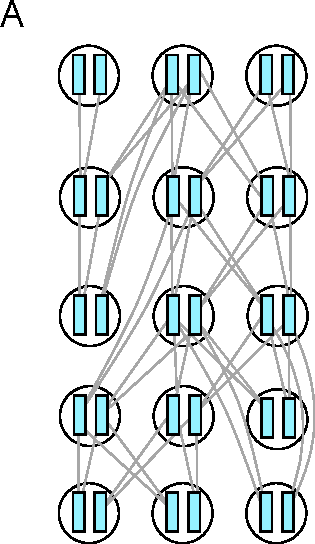
\includegraphics[width=0.3\textwidth]{figures/pedigree0.pdf}\hspace{0em}} % MFR: I added these spaces because for some weird reason Inkscape keeps crashing when I try to edit the original svgs
    \hfill
    \subcaptionbox{Those relationships left at the end of the simulation.}{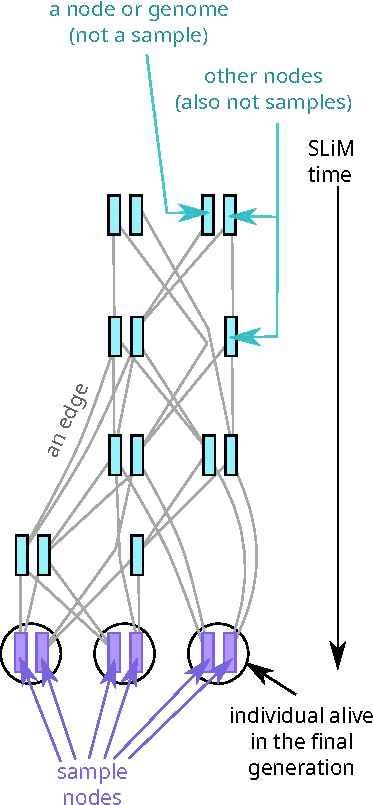
\includegraphics[width=0.3\textwidth]{figures/pedigree2.pdf}}
    \hfill
    \subcaptionbox{Additional individuals may be ``remembered'' (purple)
        or ``retained'' (dotted).}{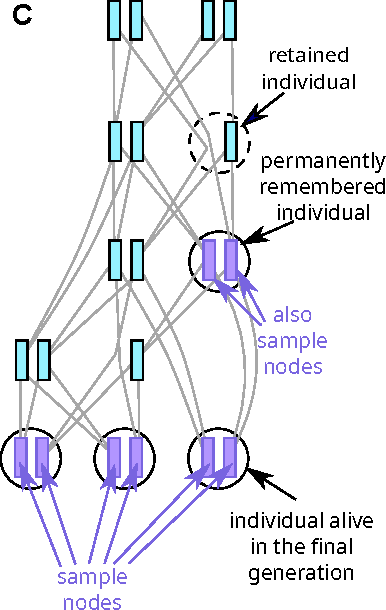
\includegraphics[width=0.3\textwidth]{figures/pedigree_remember.pdf}}
\caption{
    The resulting genetic relationships between individuals in a small simulation
    (three diploids over five generations).
}
\label{fig:indivs}
\end{figure}

\paragraph{Who is and isn't in the tree sequence:}
Suppose we have run a very small simulation with \slim. The genetic relationships among each of the
diploid individuals who were alive over the course of the simulation might
look something like Figure~\ref{fig:indivs}A. Since individuals (circles) are diploid, each contains
two genomes or nodes (shaded rectangles).
The edges of the tree sequence record which specific parts of the genome are inherited,
so the relationships recorded in the tree sequence are between the nodes and not the individuals directly.

By default, the sample nodes are simply the genomes of the individuals that are alive in the final generation
of the simulation. This renders large portions of these relationships unnecessary for representing the samples' history,
as they correspond to lineages that died out at some earlier point in the simulation (but see section below on
``Historical Individuals'' about how to record ancient samples).
To avoid having to
store this large quantity of unnecessary information, \slim periodically \textit{simplifies} the tree sequence
as the simulation goes along. By default, simplification will only keep the portions of the
genetic genealogy that are required to represent the history of the current nodes \citep{kelleher_efficient_2018}.
Additionally, it defaults to removing any node that is not a genetic
\textit{most recent common ancestor} (MRCA) of at least two daughter nodes. This removes historical
nodes that are only ``on the line to'' a sample, but do not represent a branching point
(\ie coalescent event) on the genealogical tree at some point on the genome.
(These 'unary nodes' can be retained within \slim in certain cases,
as we discuss below.)

As a result of the simplification process, the output tree sequence will look something like Figure~\ref{fig:indivs}B.
To be precise, edges correspond to inherited genomic \emph{segments} with defined start and end positions,
but we do not attempt to depict that complexity here.
% PLR: this is not true because nodes have more than one ancestor
% Instead, this figure can be thought of as representing a simulation
% with no recombination, so entire nodes, rather than genomic segments, are being inherited.

Individuals who are alive at the end of the simulation automatically have their nodes marked as
\textit{samples}. All other historical (\ie dead) individuals (depicted as circles) have vanished,\
although some of their nodes remain. As discussed previously, these nodes have only been retained because they are required to
accurately represent the ancestry of one or more sample nodes and/or the relationships among sample nodes.

%%%%%%%% %%%%%%%%%%%%%%
\section*{Historical individuals}
By default, only the nodes associated with individuals alive in the final generation are part of the set of samples.
However, there are many cases where we might want to retain the complete ancestry, and other metadata, for
historical individuals.
For example, we might want to model the relationship between a modern population and
one particular individual from the past.
Or, as below, if we are conducting simulations in parallel that share 
a common ancestry, we may need to retain certain nodes that are critical for linking distinct
tree sequences back together.
In order to accomplish this, we can choose to ``remember'' key individuals during the course of the simulation,
using the \slim function \verb|treeSeqRememberIndividuals()|.

\paragraph{Permanently remembering individuals}
By default, a call to \\ 
\verb|treeSeqRememberIndividuals()| will permanently remember one or more individuals,
the simulated equivalent of ancient DNA dug out of permafrost.
This means that any tree sequence subsequently recorded will always contain this individual,
its nodes (now marked as samples), and its full ancestry.
The result of remembering an individual in the introductory example is pictured
in Figure~\ref{fig:indivs}C.
This is also useful to, for instance, access allele frequencies and spatial locations of individuals
at a particular time in the past.
As an extreme case, all individuals at all time points can be remembered,
thus retaining the complete population pedigree of everyone ever alive,
but this quickly becomes computationally burdensome.

\paragraph{Retaining individuals}
Alternatively, you may want to only retain historical individuals as long as their nodes are still
relevant to reconstructing the genetic ancestry of the sample nodes.
The ancestral nodes that \slim includes in the tree sequence do not by default have their associated individuals included as well,
and so at the end of the simulation we do not by default have access to individual-level information for non-sample nodes
such as spatial location or parental IDs.
But, we can ask \slim to also record historical individuals (and hence their associated information)
as long as their nodes are retained through simplification.
This is less burdensome than remembering them, as individuals can still be removed once their
nodes (which are not marked as samples) are no longer ancestral.
You can \emph{retain} individuals in this way by using
\verb|treeSeqRememberIndividuals(..., permanent=F)|.
Since a retained individual's nodes are not samples,
they are subject to the standard removal 'rules' of simplification.
It is therefore possible to end up with an individual containing only one genome, as shown in the diagram.
However, as soon as both nodes of a retained individual have been lost,
the individual and any information associated with it is deleted as well.

As previously discussed, simplification will, by default, only keep nodes if they are a coalescent point
(\ie they are a MRCA or branch point) somewhere along the genome.
This can be changed by initialising tree sequence recording in \slim using
\verb|treeSeqInitialize(retainCoalescentOnly=F)|.
SLiM will then preserve all retained individuals while they remain in the genealogy of present-day individuals,
even if their nodes are not coalescent points in the tree.
If you later decide to reduce the number
of samples in the tree sequence, you can do so using the tskit function \verb|simplify()|
(which is what \slim uses under the hood).
In this case, individuals that are ``retained'' rather than ``remembered'' will be kept only
if they are still MRCAs in the ancestry of the selected samples.
To preserve them even if their nodes are not coalescent points,
you can use the \verb|keep_unary_in_individuals| argument to \verb|simplify|.

%%%%%%%%%%%%%%%%%%%%%%%
\section{Recapitation: tying up loose ends} %% "Streamlining the burn-in, two ways"

\begin{figure}
\centering
    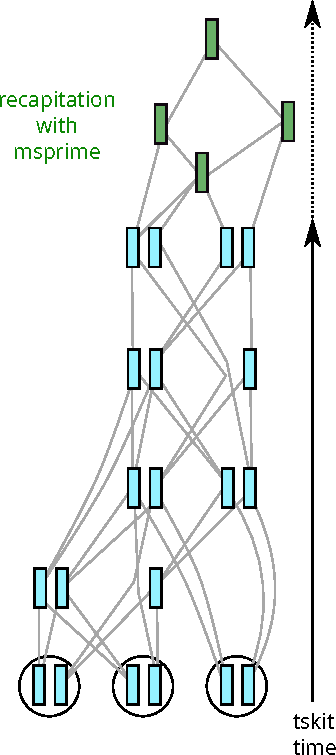
\includegraphics[width=0.2\textwidth]{figures/pedigree_recapitate.pdf}
    % 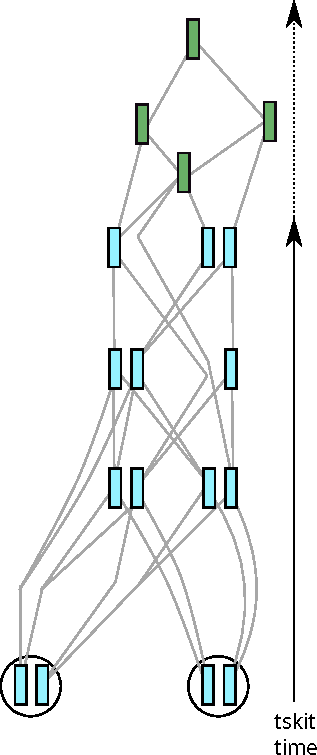
\includegraphics[width=0.2\textwidth]{figures/pedigree_simplify.pdf}
\caption{
    % \textbf{(A)}
    Recapitation adds the green nodes 
    to the simulation of Figure~\ref{fig:indivs} by coalescent simulation.
    % \textbf{(B)} The result of \emph{simplifying} the tree sequence in (A)
    % down to the four sample nodes shown.
}
\label{fig:recap_simp}
\end{figure}

By default, a \slim simulation begins with all individuals being identical, and genetic diversity
builds up over time as new mutations occur. However, in many cases, starting with a clonal population
is undesirable and can have long-lasting effects on patterns of diversity in the samples. One way to overcome
this is to include a long ``burn-in'' period in the forward simulation to reach an equilibrium level of genetic diversity.
However, this period generally needs to be quite long (on the order of 5--15 times the effective population size, in generations),
which can be prohibitive.
An efficient alternative is to ``seed'' the simulation with genetic diversity generated by a coalescent simulation, \ie conduct a hybrid simulation.
There are two main ways to do this, which we refer to as ``recapitation'' and ``generating initial diversity'', respectively.
Both ways should be thought of as generating initial diversity, but recapitation (counterintuitively) generates that diversity after the fact.
So, the main difference between them is when
this coalescent step is run relative to the forward-in-time portion of the simulation.
We will discuss these approaches in the following two sections.

Recapitation is done with a tree sequence generated by \slim simulation.
This is suitable if the \slim step does not require the ancestral genotypes for anything, such as determining individual fitness,
so all we want to know is how the demographics of the \slim simulation affects initially present neutral variation.
Functionally, recapitation conducts a coalescent simulation
starting with the those portions of the first-generation ancestral nodes (\slim time 0) that have not yet coalesced.
This is discussed in more detail in \citet{haller_tree-sequence_2019}.

Figure~\ref{fig:recap_simp} illustrates this process: imagine that, at some sites, one or more samples do not share
a common ancestor within the \slim simulated portion of history (shown in blue).
Recapitation starts at the \textit{top} of the genealogies and moves backwards in time
to fill in a genealogical history for all the samples.
The green chromosomes here are new ancestral nodes that have been added to the tree sequence.
As previously mentioned, the effect of omitting this step would be to model a genetically homogeneous initial population;
our simulation would have less genetic variation than it ``should'' have, since the all the variation
contributed by the green portion of the tree would be omitted.

% % PLR: I don't think we need this?
% It is important to consider how time is conceptualized in this hybrid simulation. In forward simulation (\ie \slim) time,
% the first-generation ancestors at the top of the blue portion of the genealogy are ``born'' at time 0. When we recapitate the genealogy,
% nodes in the green portion of the genealogy will necessarily be born in negative \slim time since they arise before the events of the
% forward-in-time portion of the simulation. In coalescent time, the age of the recapitated nodes simply increases relative to the final generation
% (\ie the set of nodes at the \textit{bottom} of the blue genealogy). %% could be explained more clearly, i think (SSG)

Recapitation within a single randomly-mating population of a size \verb|N|
can be achieved with a simple call to \verb|pyslim.recapitate(ts, ancestral_size=N)|
Since \verb|pyslim.recapitate| is a wrapper around
\verb|msprime.sim_ancestry|, we could recapitate our tree with any model that can be represented by \msprime code \citep{baumdicker_efficient_2022}.
For instance, it is possible to recapitate a \slim-generated tree sequence with a fluctuating population size
or non-uniform genetic map by simply passing in the relevant arguments.

Setting up a demographic model in \msprime that is consistent and compatible with a particular \slim simulation requires
understanding some of the finer details of each of these software packages, so here we will present a concrete example.
Suppose our \slim model has the following population structure:
\begin{minted}[fontsize=\small, linenos, bgcolor=gray!10]{slim}
1 early() {
   sim.addSubpop("p1", K);
   sim.addSubpop("p2", K);
}
\end{minted}
If the resulting tree sequence is stored in the file \texttt{recap\_example.trees},
then examining the populations using the shell, we see
(edited to remove some extraneous information):
% % what it actually looks like:
% \begin{minted}[fontsize=\small, linenos, bgcolor=gray!10]{bash}
% > tskit populations recap_example.trees
% id	metadata
% 0	None
% 1	{'migration_records': [], 'name': 'p1', 'sex_ratio': 0.0, 'slim_id': 1}
% 2	{'migration_records': [], 'name': 'p2', 'sex_ratio': 0.0, 'slim_id': 2}
% \end{minted}
\begin{minted}[fontsize=\small, linenos, bgcolor=gray!10]{bash}
> tskit populations recap_example.trees
id	metadata
0	None
1	{'name': 'p1', 'slim_id': 1}
2	{'name': 'p2', 'slim_id': 2}
\end{minted}
There are \emph{three} populations, but the first one is unused (and has no metadata),
because \slim stores population \texttt{pX} as population \texttt{X}.
To be compatible with this tree sequence, the \msprime demographic model will need to include three populations as well.
However the first population will remain unused unless we specify it as an ancestral source for
one of the other two populations during the coalescent phase of the simulation.
% Note that we could have avoided having this
% `dummy' population if we had named our two populations `p0' and `p1' within the \slim script. Similarly, if we would have started
% numbering our populations from `p3', we would end up with a total of three `dummy' populations in our tree sequence.

Regardless of the population numbering scheme used, \msprime provides a built-in method of seamlessly generating a
compatible demography given a particular starting tree sequence file. The following code uses the information in the tree sequence \verb|ts|
to create a basic compatible demography:
%% read recap_example.trees as ts?
\begin{minted}[fontsize=\small, linenos, bgcolor=gray!10]{python}
ts = tskit.load("recap_example.trees")
demography = msprime.Demography.from_tree_sequence(ts, initial_size=100)
\end{minted}
The resulting demography has 3 populations with an effective size of 100 individuals each.
Note that the \verb|initial_size|
does not have to match what we specified in our \slim simulation, because it specifies the size of the generation
immediately preceding the \slim phase. We could theoretically try to recapitate our tree sequence with this
demography, but if we did so, \msprime would run forever. This is because we have not allowed for any way for
lineages from population \p1 to coalesce with lineages in population \p2, or vice versa.
Therefore, the coalescent process will never be able to conclude.

To remedy this,
% we need to provide a migration path that allows lineages from different populations to coalesce.
let us specify one-directional migration from \p1 to \p2 (so, lineages in \p2 move into \p1 as we move backwards in time)
starting 100 generations before the start of the \slim simulation.
The current time (``tick'') in \slim is stored in the tree sequence's top-level metadata, as \verb|ts.metadata['SLiM']['tick']|,
which we can use to identify when the desired time point is
(and note that this must be specified in tskit time, \ie as ``time ago'').
\begin{minted}[fontsize=\small, linenos, bgcolor=gray!10]{python}
demography.add_migration_rate_change(
    time=ts.metadata["SLiM"]["tick"] + 100,
    rate=0.1, source="p2", dest="p1")
rts = pyslim.recapitate(ts, demography=demography,
            recombination_rate=1e-8)
\end{minted}

The \pyslim function `recapitate' passes the tree sequence \verb|ts| to the
\verb|initial_state| argument of \verb|msprime.sim\_ancestry|,
along with the demographic model that we specified.
The root of each uncoalesced lineage in this tree sequence is a node
that exists at a particular time and in a particular population;
these two things situate the lineage within the demographic model,
allowing \msprime to continue following the lineages back through time.

At this point we need to raise an important caveat:
in non-Wright-Fisher models in \slim,
time units are likely not in units of generations.
This means that \emph{different} mutation and recombination rates need to be passed to \msprime,
because these rates in \slim are ``per generation'' while for \msprime they are ``per unit time''.
For these and other considerations, see the \pyslim documentation.

%%%%%%%%%%%%%%%%%%%%%%%%%%%%%%%%%%%%%%
\section{Generating initial diversity} % is there a better name for this process? this doesn`t have the same ring as 'recapitation'

If the \slim will use genotypes present as intial diversity during the simulation,
then we cannot recapitate,
run the coalescent simulation first to generate a starting tree sequence.
This tree sequence can then be loaded into \slim where the main simulation process can proceed as normal.
This approach is useful, for instance, when simulating selection on standing variation in a large population,
where a purely forward-in-time burn-in period would be very costly in terms of time and computational resources.
% Because the genetic variation needs to exist in the population at the start of the simulation, adding
% it on after the fact via recapitation, as discussed in the previous section, is not an option.
While running a neutral coalescent burn-in is not exactly the same as a running a forward-in-time burn-in with selection,
this can be an adequate approximation (but caution is advised).

For instance,
imagine that we want to perform a lab experiment in which we take high-diversity
organisms from the wild and subject them to selection for a few dozen generations.
If we use the results of a coalescent simulation to represent our sample from the wild,
then we are effectively assuming that the genetic diversity in the wild population is (approximately) neutral.
This may not reflect reality: for instance,
alleles with larger effect on a trait under stabilizing selection might be expected to be at lower frequency.
For these reasons, we still suggest some burn-in in \slim,
although less is probably required, since you don't have to wait for diversity to be generated by mutation.
For our example, we will assume simply that the trait we are selecting for in the lab was
not under selection in the wild. To implement this, we will:
(1) run a coalescent simulation with \msprime;
(2) ``annotate'' the resulting tree sequence with \slim metadata, allowing it to be read into \slim;
(3) add \slim mutations with \msprime
        and edit the mutation metadata to assign selection coefficients; and finally
(4) run the \slim portion of the simulation.

\subsection*{Annotating a tree sequence with SLiM metadata}

Suppose we run the following coalescent simulation in \msprime:
\begin{minted}[fontsize=\small, linenos, bgcolor=gray!10]{python}
  demog_model = msprime.Demography()
  demog_model.add_population(initial_size=1_000)
  ts = msprime.sim_ancestry(
          samples=1_000,
          demography=demog_model,
          random_seed=5,
          recombination_rate=1e-8,
          sequence_length = 90_000_000)
\end{minted}
This tree sequence \verb|ts| is a complete record of the genealogical information relating specific individuals
and nodes, but is missing other information that  SLiM requires.
The other information needs to be added to metadata of various objects in the tree sequence,
and can be easily added using the \verb|annotate| function from \pyslim.
Although this function adds default values for most information,
we must provide the model type (Wright-Fisher or non-Wright-Fisher)
and some information about how coalescent- and SLiM-time\ should be aligned.
\begin{minted}[fontsize=\small, linenos, bgcolor=gray!10]{python}
ats = pyslim.annotate(ts, model_type="WF", tick=1, stage="late")
\end{minted}
When this tree sequence is loaded into \slim, the tick counter (\ie \slim time)
will be set to 1, and if it is not loaded in during the \verb|late()| stage a warning will be raised.

The function \verb|annotate()| fills in default values for every element of the tree sequence that requires it,
which includes all individuals, all nodes that exist within living individuals, and all
populations referenced by nodes. We can see exactly what these defaults
are for any given component of the tree sequence by using \verb|default_slim_metadata|,
for instance:
\begin{minted}[fontsize=\small, linenos, bgcolor=gray!10]{python}
pyslim.default_slim_metadata("individual")
# {'pedigree_id': -1, 'age': -1, 'subpopulation': -1, 'sex': -1,
#  'flags': 0, 'pedigree_p1': -1, 'pedigree_p2': -1}
\end{minted}
So, by default all individuals as hermaphroditic (individual \verb|sex| is -1)
and \verb|age| is -1 (as appropriate for a WF simulation).
If we wanted, for instance, a sexual population we would then edit these values.
Below, we show how to do this specifically for mutations, but other modifications
can be done in a similar manner.

\subsection*{Adding mutations with SLiM metadata}

The simulation thus far had no mutations, so
the next step is to generate the initial genetic diversity that natural selection will act on
in the forward-in-time phase of our hybrid simulation. Let us assume an overall rate of $3 \times 10^{-8}$ new
mutations per base pair per generation. Further, let us assume that 99\% of all new mutations
are neutral, and the remaining 1\% have a selection coefficient of 0.001.
If we were doing this simulation entirely within a forward-in-time framework with a long
burn-in, we could have achieved this outcome using the following \slim code:
\begin{minted}[fontsize=\small, linenos, bgcolor=gray!10]{slim}
        initializeMutationType("m2", 0.5, "f", 0.001);
        initializeMutationRate(3e-10);
\end{minted}
This code defines a mutation type \verb|m2| that has a dominance coefficient of 0.5 and a fixed selection
coefficient of 0.001 (the latter can be made more flexible, \eg drawn from a distribution -- see the \slim manual).
Notice, too, that we have set these non-neutral mutations to arise at a rate of $3 \times 10^{-10}$ per base per generation,
or 1\% of our desired overall mutation rate of $3 \times 10^{-8}$,
so we would add the remaining neutral mutations after the fact (as we do below here as well).
To approximate this result using \msprime, we must first
use the function \verb|msprime.sim_mutations|
with the \verb|SLiMMutationModel| to generate some mutations on the existing tree sequence:
\begin{minted}[fontsize=\small, linenos, bgcolor=gray!10]{python}
mut_model = msprime.SLiMMutationModel(type=2)
mts = msprime.sim_mutations(ats, rate=3e-10, model=mut_model)
\end{minted}
The \verb|type=2| argument denotes that the mutations will be of type \verb|m2| in SLiM, which will also
need to be explicitly initialized in the forward-in-time phase of the simulation (as in the \slim code above).
By default, these mutations are assigned a selection coefficient of 0, which is accurate since they
all arose in the neutrally-evolving portion of the tree. However, since we want selection to come into
effect for the \slim phase, we will need to update the selection coefficients of these variants.
Tree sequences are, for efficiency purposes, not directly modifiable. Therefore, to update any aspect of
a particular tree sequence we need to instead copy its underlying tables, modify them,
and then re-generate the tree sequence.
Doing this to change all selection coefficients to 0.001 looks like this:
\begin{minted}[fontsize=\small, linenos, bgcolor=gray!10]{python}
tables = mts.dump_tables()
tables.mutations.clear()
for m in mts.mutations():
  md_list = m.metadata["mutation_list"]
  for md in md_list:
    md["selection_coeff"] = 0.001
    tables.mutations.append(
        m.replace(metadata={"mutation_list": md_list})
    )

sts = tables.tree_sequence()
\end{minted}
This code first copied all the tables that describe the tree sequence \verb|mts|, cleared all the
information in the mutations table, and then added each existing mutation from \verb|mts| back with a new selection
coefficient. Finally, it generated a new tree sequence from the resulting, modified, tables.
This tree sequence can now be read into \slim in order to proceed with the forward-in-time phase of our coalescent simulation.

Before we proceed to that step, however, we should take a detour through
some details about how mutations are represented in both \slim and \tskit. 
This is necessary to understand the above code (what is \verb|mutation_list|?),
and it has potentitally confusing implications for hybrid simulations. 
In \tskit, each mutation has a ``derived state'', which is the allelic state that completely replaces any previous allelic state.
So, if a mutation occurs at a site where a mutation already exists,
the most recent mutation will replace the older one.
This differs from \slim, which, by default, allows recurrent mutations at the same genomic
position to `stack' on top of each other.
So, the \verb|SLiMMutationModel| encodes this ``stacking'' information within the \tskit mutation object.
Consider the following example of a `double hit' mutation
that could have been produced by the code above, produced by \verb|print(sts.mutation(295))|
(it is the $295^\text{th}$ mutation in \verb|sts|):
\begin{minted}[fontsize=\small, linenos, bgcolor=gray!10]{python}
Mutation(id=295, site=180, node=43931, derived_state='193,194',
   parent=294, time=8.74,
   metadata={'mutation_list': [
      {'mutation_type': 2, 'selection_coeff': 0.001, 'subpopulation': -1, 'slim_time': -559, 'nucleotide': -1},
      {'mutation_type': 2, 'selection_coeff': 0.001, 'subpopulation': -1, 'slim_time': -7, 'nucleotide': -1}
   ]} )
\end{minted}
There are two parts of this record that give away the fact that this was a recurrent mutation.
First, the \verb|derived_state| is a comma-separated list of \emph{two} integers, \verb|193,194|.
These integers are the \slim IDs of the corresponding mutations.
Second, the \verb|mutation_list| element of the mutation's metadata has two entries which represent those two \slim mutations,
the first (with \slim ID 193) one occurring 559 ticks ago and the second (with \slim ID 194)  occurring 7 ticks ago.
% This allows \slim to reconstruct these events in order
% to apply the appropriate stacking policy if this tree sequence is used as an initial state for a forward-in-time simulation.
% So, for example,
% we can infer that a mutation occurred at this site at \verb|slim_time| $-559$ producing a derived state of 193, and then another mutation
% occurred at the same site at \verb|slim_time| $-7$ producing a derived state of 194.
If another mutation occurred later at this site on a genome carrying this mutation,
it would be recorded as a separate mutation in the mutation tables,
with derived state and mutation list having three entries each.
This is why, when modifying
the selection coefficients of each mutation earlier in this section, we had to have two nested loops --
one iterated over mutations,
while the second updated each element of the mutation's associated \verb|mutation_list|.

Sharp-eyed readers will note that the ``time'' of the mutation given by the tree sequence (8.74 generations ago) does not exactly
correspond to the \verb|slim_time| recorded in metadata ($-7$ generations in the future); in general this conversion is ``rounded and sometimes
off by one, depending on the model type''. For a detailed discussion of how time is converted between the tree sequence and the SLiM
model, see the \pyslim documentation.

\subsection*{Loading into SLiM}

We can finally move on to the forward-in-time component of our hybrid simulation.
First, suppose we have written out the tree sequence from the previous section to file
using \verb|sts.dump("init.trees")|.
We need to ensure that everything matches
between the tree sequence and the initialization of the \slim recipe we will use to load the file.
Specifically, the model type must match what we specified in the tree sequence's metadata;
the genome length must be equal to the tree sequence's \verb|sequence_length|,
and each mutation type used in the tree sequence must be declared (above, we used \verb|m2|).
In the script we will also define a placeholder mutation type \verb|m1| for neutral mutations, to be added later.
There is no need to set up a population or individuals -- this is read in from the tree sequence.
% % PLR: no need to do this?
% but we will make a point to ``Remember'' all the individuals who are alive at the start of the simulation to facilitate downstream analysis.
\begin{minted}[fontsize=\small, linenos, bgcolor=gray!10]{slim}
initialize()
{
    initializeSLiMModelType("WF");
    initializeTreeSeq();
    initializeMutationRate(3e-10);
    initializeMutationType("m1", 0.5, "f", 0.0);
    initializeMutationType("m2", 0.5, "s", 0.001);
    initializeGenomicElementType("g1", m2, 1.0);
    initializeGenomicElement(g1, 0, L-1); // specify L, the genome length
    initializeRecombinationRate(1e-8);
}
1 late() { 
    sim.readFromPopulationFile("init.trees");
}
100 late() {
    sim.treeSeqOutput("final.trees");
}
\end{minted}
This \slim code picks up the simulation where \msprime left off, applying the same mutation rate and recombination rates
for an additional 100 generations.
However, in this phase, an individual's genetic make-up (\ie the non-neutral genetic variants they carry)
will influence their fitness as the population continues to evolve.

\section{Generating realistic genetic data}

Next, we will discuss some final steps for generating a genetic dataset from our hybrid simulation that has many of the properties of real data that is generated from
sequencing or genotyping real organisms. Whether it was generated by recapitation or by first generating initial
diversity with a coalescent simulation, the following steps are necessary for adding realistic levels of neutral diversity and for ultimately producing a
file that can be analyzed by standard methods.

\subsection*{Overlaying neutral mutations}
In our two previous sections outlining the two main methods of performing a hybrid simulation, we did not bother to add neutral mutations to the tree sequence.
This is because neutral mutations do not impact the shape of the genealogy, and so adding them after the fact is equivalent to tracking them as the
simulation proceeds;
it is more efficient because it relieves \slim of the burden of tracking these irrelevant variants.
%% if you simulated neutral mutations in your SLiM phase, you'd want to be careful about adding mutations again in this phase - you'd end up with 2x rate in the SLiM portion only
In the ``Generating initial diversity'' section above, we stated that we wanted simulate an overall mutation rate of $3 \times 10^{-8}$,
with 99\% of the resulting mutations neutral.
We already added the 1\% of non-neutral mutations, so now, we need to add neutral mutations at a rate of $0.99 \times 3 \times10^{-8}$.
We will set the mutation ``type'' to 1 so that we can easily distinguish neutral and non-neutral
mutations on this property (recall that non-neutral mutations were of type 2),
matching the preamble of the \slim script above.
The first step is to load the tree sequence output by SLiM:
\begin{minted}[fontsize=\small, linenos, bgcolor=gray!10]{python}
ts = tskit.load("final.trees")
next_id = pyslim.next_slim_mutation_id(ts)
mut_model = msprime.SLiMMutationModel(type=1, next_id=next_id)
vts = msprime.sim_mutations( ts, rate=0.99 * 3e-8,
        model=mut_model, keep=True)
\end{minted}
We use \pyslim's \verb|next_slim_mutation_id| to identify the \slim mutation ID for \msprime to pick up from,
which is important as all \slim mutation IDs in the tree sequence must be unique.
Additionally, we include \verb|keep=True| so that existing mutations are not discarded.

\subsection*{VCF output}
The final step we demonstrate is to output the SLiM-coded genotype information as a Variant Call Format (VCF) file.
Doing so requires remapping some of the information to a form that resembles real genetic data.
For example, the \slim mutation model encodes the ancestral state of every site as the empty string and the derived state
as a comma-separated list of integers (also stored as a string).
These states are meaningful for \slim but do not correspond to the nucleotides expected in a VCF.
To address this, \pyslim provides functions to convert \slim mutations to a more conventional format:
first, \verb|generate_nucleotides| adds nucleotides to non-nucleotide models under a Jukes-Cantor model,
and second, \verb|convert_alleles| replaces the comma-separated lists of integers in the ancestral and derived states of the tree sequence
with the corresponding nucleotides.
% Since we started with the code above, we had to do both steps;
% if in \slim we had used a nucleotide mutation model, then the first step would not have been necessary.
Following these steps, \tskit's method \verb|write_vcf| can be used to output the VCF
(and the method itself provides more options):
\begin{minted}[fontsize=\small, linenos, bgcolor=gray!10]{python}
nts = pyslim.generate_nucleotides(vts)
nts = pyslim.convert_alleles(nts)
with open('nucs.vcf', 'w') as f:
    nts.write_vcf(f)
\end{minted}
This simply assigns each position a randomly chosen nucleotide,
and then assigns each mutation a nucleotide chosen randomly out of the three that are different
from the previous state (\ie from the Jukes-Cantor model).
More complex models could be implemented in python.

% % PLR: I don't think the following is necessary, or maybe even entirely accurate? Genotype information isn't "changed" really,
% % although the 0|1 sort of information that's printed out by write_vcf() might be? The complicated caveats around non-uniqueness
% % only apply if some mutations already have nucleotides and some don't, which is something we probably don't want to get into?
% If we compare the output of this process to a VCF file generated from the unconverted tree sequence, we can see that all previously empty ancestral states and
% all integer value derived states have been assigned a specific nucleotide.
% In the case of recurrent mutation, the \verb|generate_nucleotides| function aims to assign a unique
% nucleotide to each derived allele, but under certain specific circumstances
% this is no longer possible. It is important to note that the genotype information associated with each specific individual is
% sometimes changed by this operation.

\section{Parallelizing forward-in-time simulations of multiple species}

We have thus far demonstrated how to combine backwards- and forwards-in-time simulations
in two different ways.
Now, we will discuss how to distribute the computational load of a highly complex forward-in-time simulation across multiple processes operating in parallel,
by simulating different branches of a phylogeny independently
and stitching the resulting tree sequences together.
This approach can drastically reduce overall clock time and the memory requirements of a large phylogenetic simulation.
The main challenge with this approach then becomes
determining how to stitch together multiple ARGs that represent the same time span.

The idea works because if there is no migration between species,
any two branches stemming from the same node in a given tree do not affect each other,
and thus can be simulated in parallel.
Figure~\ref{fig:phylo} shows the simple example we work with.

\begin{figure}[h!]
    \centering
     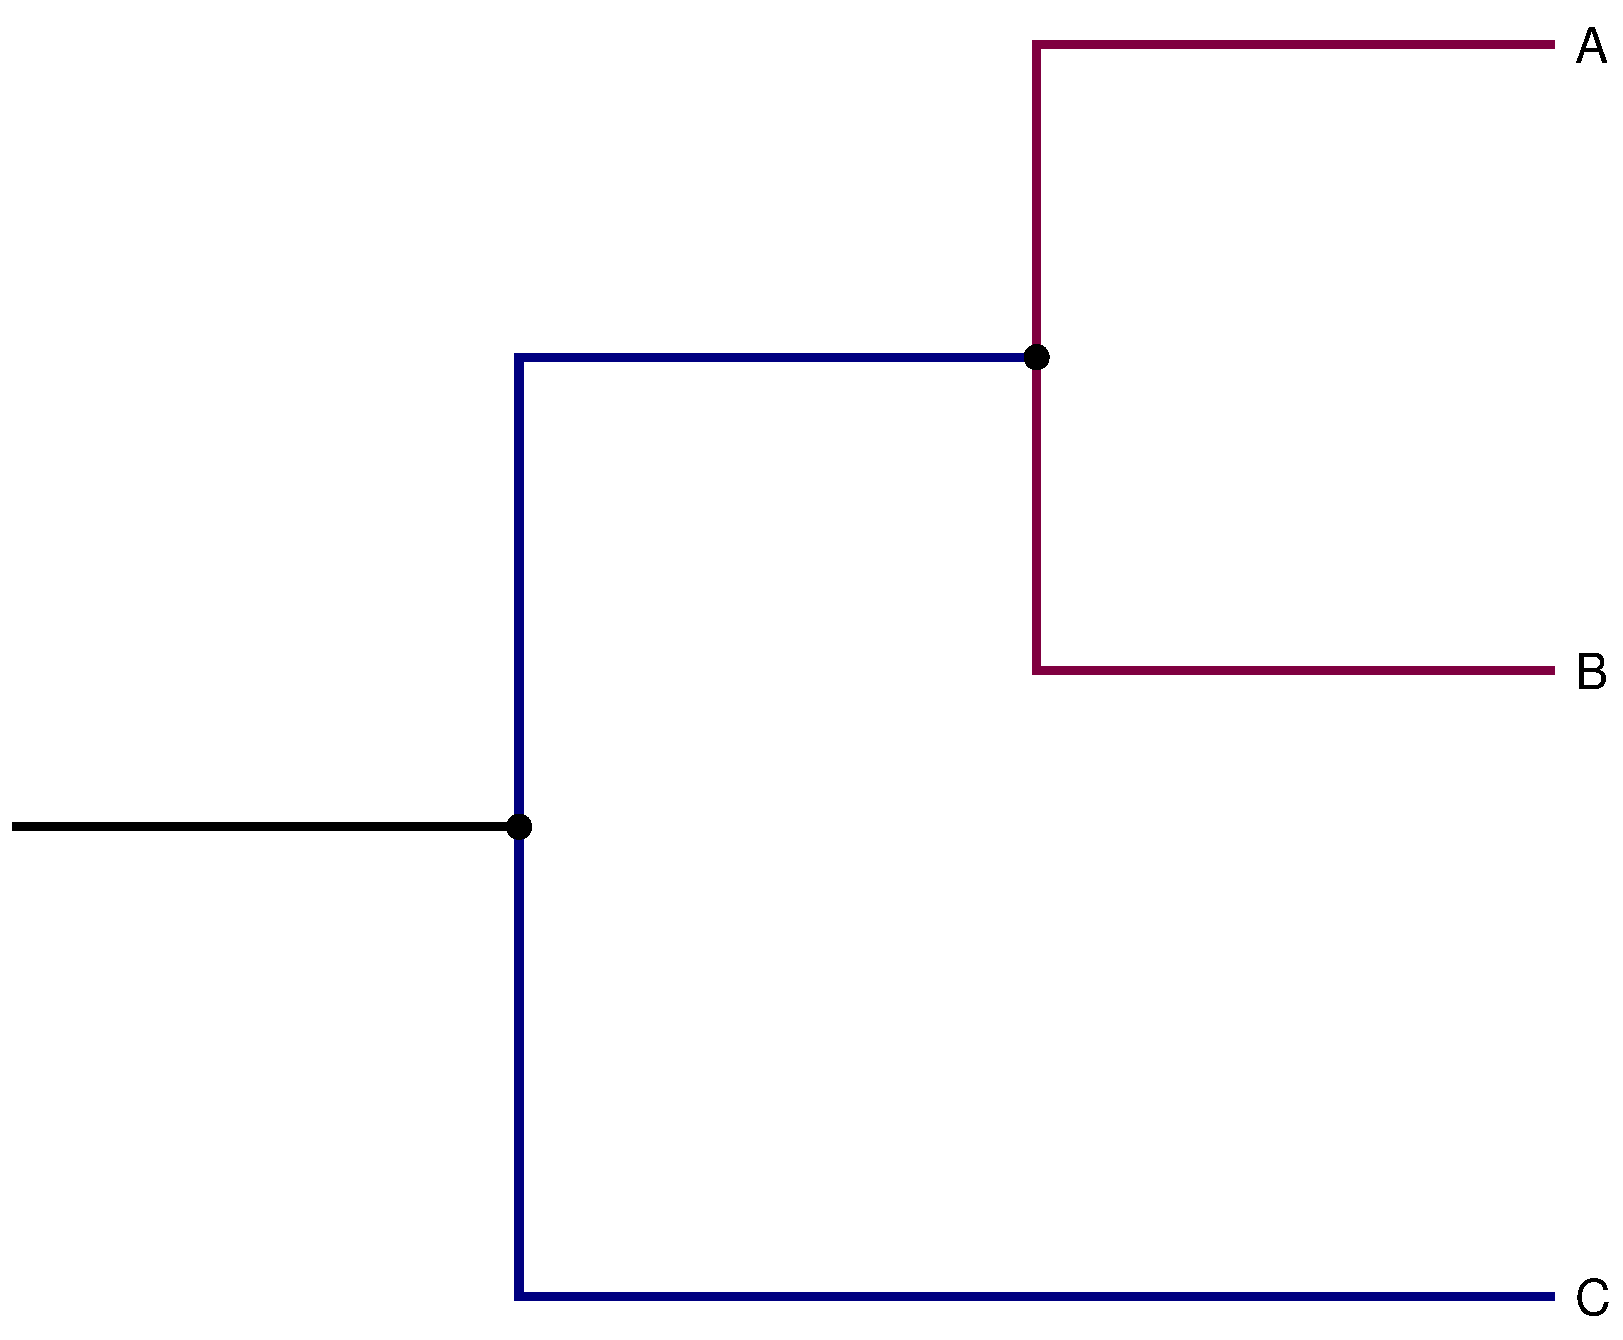
\includegraphics[width=0.33\textwidth]{code/parallelizing_phylogeny/phylo.pdf}
     \caption{
         Example phylogeny.
         Branches with the same color can be simulated in parallel if there is no migration between them.
     }
     \label{fig:phylo}
\end{figure}

\subsection{Parallel simulation of branches}

We will use the following \slim script to simulate the history of each species, represented by its own branch, in our phylogeny. Here, each species can have a different
(but fixed) population size (\verb|popsize|) and total duration (\verb|num_gen|). Additionally, we will model deleterious mutations accumulating across the entire genome at a fixed rate.
%
\inputminted[breaklines, breakautoindent=true, breakanywhere=true, fontsize=\small, linenos, bgcolor=gray!10]{slim}{code/parallelizing_phylogeny/simulate_branch.slim}
%
Notice that, in addition to \verb|popsize|, \verb|popname| and \verb|num_gen|, the variables \verb|infile| and \verb|outfile| are left undefined in this SLiM script.
This allows the relationship between branches, and the
resulting tree sequences, to be explicitly defined. As a result, this single SLiM model can represent every species simply by passing the appropriate values of \verb|infile| and \verb|outfile|.
When initializing a SLiM simulation using an existing tree sequence, the starting tick is updated
based on the time specified in the tree sequence's metadata, as seen above.
Therefore, we define the ending tick of the simulation as the start time plus the \verb|num_gens| argument.

% % PLR: I don't think we use this table?
% We can do this by recoding the phylogeny depicted in Figure~\ref{fig:phylo} as a table:
% \begin{table}[h]
%   \centering
%   \caption{Parameters of the phylogeny that will be simulated.}
%   \label{tab:phylo}
%     \begin{tabular}{llll}
%       \bfseries Child & \bfseries Parent & \bfseries Population size & \bfseries Edge length \\
%       \hline
%       \csvreader[head to column names]{code/parallelizing_phylogeny/phylo.csv}{}%
%         {\child & \parent & \popsize & \edgelen\\}
%     \end{tabular}
% \end{table}
% For each branch, the presence or absence of \verb|infile| tells \slim whether a previous branch exists or not. For the \verb|root| branch of our phylogeny, there is no \verb|parent|; this is the branch
% that is ancestral to all other branches. For all other branches, \slim will read in the \verb|parent| tree sequence and use the living individuals to create a new population, adjusting the
% final population size based on the corresponding value in the table. 

%%%% not sure that remembering is actually necessary in this case
At the end of the simulation, we call \verb|sim.treeSeqRememberIndividuals| right before saving the resulting tree sequence.
This is necessary to ensure that the individuals in the final generation are never dropped from any of the future runs that are started from this simulation's output,
as they may be needed later to merge the tree sequences generated from parallel runs back together.
%%%%

To actually run our parallelized simulation, we could use workflow management software, such as Make or Snakemake, or a custom script -- see the \pyslim
\href{https://tskit.dev/pyslim/docs/latest/vignette_parallel_phylo.html}{documentation} for details on different implementations. Here, we will use the simple Make script below to pass
the appropriate parameters to our generic \verb|simulate_branch.slim| script.
%
\inputminted[breaklines,fontsize=\small, breakanywhere=true, breakautoindent=true, linenos, bgcolor=gray!10]{basemake}{code/parallelizing_phylogeny/parallel_sims.make}
%
This script essentially recodes our original phylogeny through a list of `rules' that define each parent-child relationship.
For example, the files `A.trees' and `B.trees' both depend on the internal node `I.trees',
which in turn depends on the result of simulating the ultimate ancestral branch `root.trees'.
Each rule in the Make file also specifies how to generate the output given the required input through a single line of SLiM code.

We can then run these simulations in parallel by executing the following bash code,
in which the -j argument specifies the maximum number of simulations to run simultaneously:
\begin{minted}[fontsize=\small, linenos, bgcolor=gray!10]{bash}
make -f sims.make -j 3
\end{minted}

\subsection{Putting it back together: unioning the tree sequences}

We now need to stitch the resulting tree sequences back together.
Remember, each of the tree sequences representing species `A', `B', and `C'
are distinct, but overlap significantly as a result of their shared evolutionary history.
To join them together, we need to specify which bits are shared and which are not.
This can be accomplished for pairs of tree sequences using the \verb|union| operation from \tskit,
which simply copies the unique parts of one of the tree sequence onto the other.
Figure~\ref{fig:union} illustrates how this works.

\begin{figure}[h!]
    \centering
     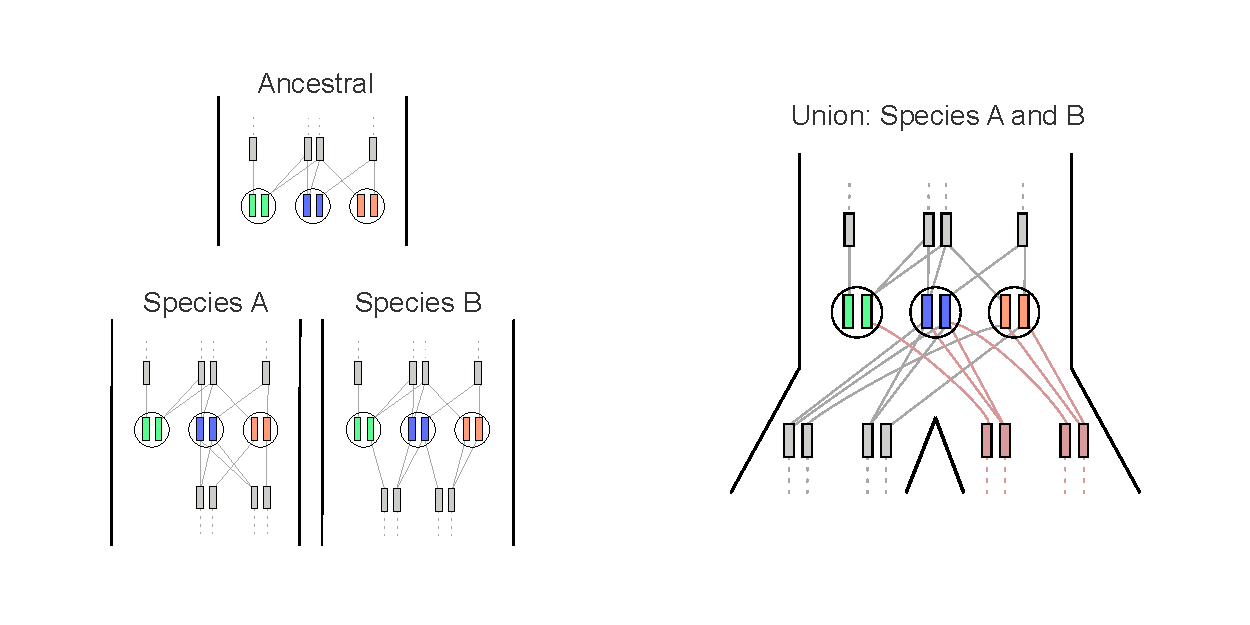
\includegraphics[width=\textwidth]{figures/union.pdf}
     \caption{
         Species A and B share the same ancestral history, but after the split they are simulated independently. Note how the history above the split (delimited by the individuals which are remembered and persistent across tree sequences, highlighted in green, blue and orange) is identical.
     \tskit's \texttt{union} operation will merge these tree sequences given a mapping that communicates which nodes in the two tree sequences are the same.
     In this example, union would add to A any new history found in B;
     these new nodes and relationships are shown in light red in the result.
     \label{fig:union}
     }
    \end{figure}

The key to correctly combining a given pair of tree sequences is to identify which parts of each are shared between the two.
To do that, \verb|union| requires a `map' that matches shared nodes across the two tree sequences.
Using this map, \verb|union| (a) checks that any properties of shared nodes and relationships between them are identical, and
(b) appends any new nodes and relationships found in the second tree sequence to the first one.
Luckily, \slim stores a value called \verb|slim_id| in the metadata of each node that it produces,
which we can use to identify the shared nodes.
However, a matching \verb|slim_id| is not sufficient to identify a positive match,
because although \verb|slim_id| values are unique within a given \slim simulation,
the same IDs will be used in different (parallel) simulation.
When \slim loads a tree sequence in order to continue a simulation,
it will start assigning \verb|slim_id| values to new nodes using the last \verb|slim_id| value
present in the ancestral tree sequence as a starting point.
so, when more than one simulation is initiated with the same
ancestral tree sequence and the resulting tree sequences are merged back together, it is likely for the same \verb|slim_id| to be used to refer to different nodes.
However, we can use node \emph{time} to resolve the issue:
referring to Figure~\ref{fig:union}, if two nodes that were born before the split time between `A' and `B'
have the same \verb|slim_id|, then they must represent the same ancestral genome (and so must have exactly the same time);
while if they were born after the split time, they represent different ancestral genomes.
The following function constructs a ``node map'' that identifies the nodes shared by two tree sequences, \verb|other| and \verb|ts|,
by identifying pairs of nodes that arose before \verb|split_time| and have the same \verb|slim_id|.
The output is an array with one value for each node in \verb|other|,
whose \verb|j|th entry is the ID of the matching node in \verb|ts| if the node is shared.,
or else is \verb|-1| otherwise.
This code could be made easier to read by iterating over nodes,
but the following numpy-based version is much faster:
%    """
%    Given SLiM tree sequences `other` and `ts`, builds a numpy array with length
%    `other.num_nodes` in which the indexes represent the node id in `other` and the
%    entries represent the equivalent node id in `ts`. If a node in `other` has no
%    equivalent in `ts`, then the entry takes the value `tskit.NULL` (-1). The
%    matching is done by comparing the IDs assigned by SLiM which are kept in
%    node metadata. This matching of SLiM IDs is *only* done for nodes with time
%    older than the specified `split_time`.
%    """
\begin{minted}[fontsize=\small, linenos, bgcolor=gray!10]{python}
def match_nodes(other, ts, split_time):
    node_mapping = np.full(other.num_nodes, -1, dtype='int')
    ts_ids = np.array([n.metadata["slim_id"] for n in ts.nodes()])
    other_ids = np.array([n.metadata["slim_id"] for n in other.nodes()])
    alive_before_split1 = (other.tables.nodes.time >= split_time)
    shared_id = np.isin(other_ids, ts_ids)
    both = np.logical_and(alive_before_split1, shared_id)
    sorted_ids = np.argsort(ts_ids)
    matches = np.searchsorted(
        ts_ids,
        other_ids[both],
        side='left',
        sorter=sorted_ids
    )
    node_mapping[both] = sorted_ids[matches]
    return node_mapping
\end{minted}
This node map can then be used with \verb|ts.union| to combine our tree sequences pairwise.
A general-purpose recursive strategy to do this is provided in the \pyslim documentation,
but the problem is easy in this simple example:
\begin{minted}[fontsize=\small, linenos, bgcolor=gray!10]{python}
    A, B, C = (tskit.load(f"{x}.trees") for x in ['A', 'B', 'C'])
    nm = match_nodes(B, A, split_time=50)
    AB = A.union(B, nm)
    nm = match_nodes(C, AB, split_time=200)
    ABC = AB.union(C)
\end{minted}
% 
% The following recursive function through the data frame containing the phylogeny and returns a dictionary
% describing a series of merging steps from tip to root.
% For a simple example such as the one we describe here, this could be done easily by hand; however, the following function
% is more flexible and will work even for complex cases.
% \begin{minted}[fontsize=\small, linenos, bgcolor=gray!10]{python}
% merged = {
%     row.child : {
%         "ts": tskit.load(row.outfile),
%         "depth": row.edgelen,
%         "children": [row.child]
%     }
%     for i, row in df[df.is_leaf].iterrows()
% }
% 
% def union_children(parent, df, merged):
%     print(f"Going in: {parent}")
%     child_rows = df[df.parent == parent]
%     assert (len(child_rows) == 2) or (len(childs) == 0)
%     if len(child_rows) == 2:
%         children = [row.child for _, row in child_rows.iterrows()]
%         for child in children:
%             if child not in merged:
%                 union_children(child, df, merged)
%         split_time = merged[children[0]]["depth"]
%         assert split_time == merged[children[1]]["depth"] # ultrametric
%         print(f'Unioning: {children}, Split time: {split_time}')
%         ts0 = merged[children[0]]["ts"]
%         ts1 = merged[children[1]]["ts"]
%         node_map = match_nodes(ts1, ts0, split_time)
%         tsu = ts0.union(ts1, node_map)
%         # the time from tip to start of simulation is split_time plus the
%         # length of the edge
%         parent_edgelength = df[df.child==parent].edgelen.item()
%         merged[parent] = {
%             "ts": tsu,
%             "depth": split_time + parent_edgelength,
%             "children": merged[children[0]]["children"] + merged[children[1]]["children"]
%         }
% 
% union_children("root", df, merged)
% # union of all three species tree sequences is in the root.
% tsu = merged["root"]["ts"]
% pops = merged["root"]["children"]
% \end{minted}
% 
The result of executing this code is a single tree sequence,
\verb|ABC|,
that fully represents the genealogy of the sampled individuals from all three extant species in our phylogeny (Figure~\ref{fig:phylo}).
Because each branch of the tree was modeled as a distinct population and SLiM, it is straightforward to identify which nodes and individuals belong
to which branch on the phylogeny throughout time.
After potentially recapitating and adding neutral mutations, we could analyze this tree sequence
like any other to answer a variety of questions related to the evolutionary history and genetic ancestry of these species.
% For example, by running multiple replicates of this
% simulation, we could achieve a reasonable expectation of the rate of incomplete lineage sorting under these specific demographic parameters.

The major advantage of running simulations in parallel is that it expands the scope for complexity and size of feasible models.
We can simulate many more species, or much larger
populations within those species, if we can split the computational burden in this way.
For example, \citet{rodrigues_shared_2024} used this parallelized approach to conduct
whole-chromosome simulations of the entire history of great apes spanning over 10 million years.
In this case, some individual species simulations used over 100Gb of memory,
and so without parallelization, simulating great apes species history in a single process would have been effectively impossible given the current limitations on computational resources.


%%%%%%%%%%%%%%%%%%%%%%%%%
\section*{Discussion}

Moving from simulation of genotype data to full ARGs presents may opportunities for evolutionary genomic inference.
ARGs can store a great deal more information about a population's evolutionary history,
while making simulation more efficient \citep{kelleher_efficient_2018}.
Furthermore, as we discuss here, information can also be passed between different simulations via the ARG,
which enables hybrid simulations that combine both forward- and backward-in-time components as well as parallel simulations.
In this chapter, we have sought to introduce readers to these method's potential to expand the scope of evolutionary simulation.
Additionally, we have provided practical vignettes that use \pyslim,
a software package that provides functions to make model interoperability between \slim and \tskit more seamless.

% Time units
In this paper, we have opted to cover opportunities and strategies more than technical detail,
and so for some technical aspects, advanced users will need to consult the documentation.
One important aspect is \emph{time units}:
we alluded to the fact that time units in \slim and \tskit differ in direction,
and that exact conversion between them can be difficult:
it depends on the stage in the \slim model.
More importantly, for non-Wright-Fisher models in \slim, a single tick may not necessarily equal one generation,
so recombination or mutation rates may need to be adjusted.
The topic is covered in more detail in the \pyslim documentation.

An overarching theme here, and for evolutionary simulations more generally, is the trade-off between realism and efficiency.
Forward-in-time simulations can be fashioned to more naturally match real population dynamics,
but this generally comes at the cost of speed. On the other hand, coalescent simulations make many assumptions, many of which
are unrealistic, in exchange for faster runtimes.
The same trade-off occurs when considering rescaling \citep{cury_simulation_2022,dabi_population_2025}.
In this paper, we describe how users can begin to achieve the best of both worlds,
outlining several examples that leverage hybrid approaches and parallelization to model scenarios that would otherwise be
computationally intractable.

While approximations are always necessary in modeling, advances in simulation and ARG software have gone along way to increase realism.
For example, we discuss how we
can use a coalescent phase to reduce the burden of simulating a burn-in period.
As a result, ancient events occur under a much less realistic model, but this may be acceptable in certain situations.
As with all cases where the validity of a particular approximation may be questionable, a good strategy is to adjust its parameters
(\eg the duration of the forward-in-time phase prior to recapitation) to see if important conclusions are affected.



%% THE END :)


%%%%%%%%%%%%%%%%%%%%%%%%%
\section*{Author contributions}


\bibliographystyle{plainnat}
\bibliography{references.bib}

%%%%%%%%%%%%%%
\newpage
\appendix

\end{document}

\comment{STUFF WE MAYBE DON'T WANT: moved here from above:}

\comment{Remove ILS thing and just add a paragraph citing Rodrigues et al and saying why this would be faster and would split the memory requirements across a bunch of processes.}

\section{Recapitation}


Doing this is as simple as:

\begin{minted}[fontsize=\small, linenos, bgcolor=gray!10]{slim}
orig_ts = tskit.load("example_sim.trees")
rts = pyslim.recapitate(orig_ts,
            recombination_rate=1e-8,
            ancestral_Ne=200, random_seed=5)
\end{minted}
The warning is harmless; it is reminding us to think about generation time
when recapitating a nonWF simulation (a topic we'll deal with later).

We can check that this worked as expected, by verifying that after recapitation
all trees have only one root:
\begin{minted}[fontsize=\small, linenos, bgcolor=gray!10]{slim}
orig_max_roots = max(t.num_roots for t in orig_ts.trees())
recap_max_roots = max(t.num_roots for t in rts.trees())
print(f"Maximum number of roots before recapitation: {orig_max_roots}\n"
      f"After recapitation: {recap_max_roots}")
\end{minted}

The `.recapitate` method
is just a thin wrapper around `msprime.sim\_ancestry`,
and you need to set up demography explicitly - for instance, in the example above
we've simulated from an ancestral population of ``Ne=200`` diploids.
If you have more than one population,
you must set migration rates or else coalescence will never happen.
% (see [](sec_recapitate_with_migration) for an example, and {func}`.recapitate` for more).

(TODO: mention about how to recapitate with a nonuniform map, as in the docs?)


\section{Simplification}


Probably, your simulations have produced many more fictitious genomes
than you will be lucky enough to have in real life,
so at some point you may want to reduce your dataset to a realistic sample size.
We can get rid of unneeded samples and any extra information from them by using
an operation called *simplification* (this is the same basic approach that SLiM
implements under the hood when outputting a tree sequence).

Depicted in Figure~\ref{fig:recap_simp}B is the result of applying an explicit call to
simplify to our example tree sequence.
In the call we asked to keep only 4
genomes (contained in 2 of the individuals in the current generation). This has
substantially simplified the tree sequence, because only information relevant to the
genealogies of the 4 sample nodes has been kept. (Precisely, simplification retains only
nodes of the tree sequence that are branching points of some marginal genealogy -- see
CITE % [Kelleher et al 2018](https://doi.org/10.1371/journal.pcbi.1006581) for details.)
While simplification sounds very appealing - it makes things simpler after all -
it is often not necessary in practice, because tree sequences are very compact,
and many operations with them are quite fast.
(It will, however, speed up many operations, so if you plan to do a large number of simulations,
your workflow could benefit from early simplification.)
So, you should probably not make simplification a standard step in your workflow,
only using it if necessary.

It is important that simplification - if it happens at all -
either (a) comes after recapitation, or (b) is done with the
``keep\_input\_roots=True`` option.
This is because simplification removes some of the
ancestral genomes in the first generation,
which are necessary for recapitation,
unless it is asked to "keep the input roots".
If we simplify without this option before recapitating,
some of the first-generation blue chromosomes in the figure on the right
would not be present, so the coalescent simulation would start from a more recent point in time
than it really should.
As an extreme example, suppose our SLiM simulation has a single diploid who has reproduced
by clonal reproduction for 1,000 generations,
so that the final tree sequence is just two vertical lines of descent going back
to the two chromosomes in the initial individual alive 1,000 generations ago.
Recapitation would produce a shared history for these two chromosomes,
that would coalesce some time longer ago than 1,000 generations.
However, if we simplified first, then those two branches going back 1,000 generations would be removed,
since they don't convey any information about the shape of the tree;
and so recapitation might produce a common ancestor more recently than 1,000 generations,
which would be inconsistent with the SLiM simulation.

After recapitation,
simplification to the history of 100 individuals alive today
can be done with the {meth}`tskit.TreeSequence.simplify` method:
\begin{minted}[fontsize=\small, linenos, bgcolor=gray!10]{slim}
import numpy as np
rng = np.random.default_rng(seed=3)
alive_inds = pyslim.individuals_alive_at(rts, 0)
keep_indivs = rng.choice(alive_inds, 100, replace=False)
keep_nodes = []
for i in keep_indivs:
  keep_nodes.extend(rts.individual(i).nodes)

sts = rts.simplify(keep_nodes, keep_input_roots=True)
\end{minted}

Note that you must pass simplify a list of \textit{node IDs}, not individual IDs.
Here, we used the `.individuals\_alive\_at` method to obtain the list
of individuals alive today.
Also note that there are *still* more than 100 individuals remaining - 15 non-sample individuals
have not been simplified away,
because they have nodes that are required to describe the genealogies of the samples.
(Since this is a non-Wright-Fisher simulation,
parents and children can be both alive at the same time in the final generation.)



\section{Adding neutral mutations to a SLiM simulation}

% ```{figure} _static/pedigree_mutate.png

If you have recorded a tree sequence in SLiM, likely you have not included any neutral mutations,
since it is much more efficient to simply add these on afterwards.
To add these (in a completely equivalent way to having included them during the simulation),
you can use the `msprime.sim\_mutations` function, which returns a new tree sequence with additional mutations.
Continuing with the cartoons from above, these are added to each branch of the tree sequence
at the rate per unit time that you request.
We'll add these using the {class}`msprime.SLiMMutationModel`, so that the file can be read back into SLiM,
but any of the other mutation models in msprime could be used.
This works as follows:
\begin{minted}[fontsize=\small, linenos, bgcolor=gray!10]{slim}
next_id = pyslim.next_slim_mutation_id(sts)
ts = msprime.sim_mutations(
           sts,
           rate=1e-8,
           model=msprime.SLiMMutationModel(type=0, next_id=next_id),
           keep=True,
)
\end{minted}


What's going on here? Let's step through the code.

\begin{enumerate}
    \item The mutation ``rate = 1e-8``, which adds mutations at a rate of $10^{-8}$ per bp.
    Unlike previous versions of msprime, this adds mutations using a discrete-sites model,
    i.e., only at integer locations (like SLiM).

\item We're passing ``type=0`` to the mutation model.
    This is because SLiM mutations need a "mutation type",
    and it makes the most sense if we add a type that was unused in the simulation.
    In this example we don't have any existing mutation types, so we can safely use ``type=0``.

\item We also add ``keep = True``, to keep any existing mutations.
    In this example there aren't any, so this isn't strictly necessary,
    but this is a good default.

\item If there are existing SLiM mutations on the tree sequence we need to
    make sure any newly added mutations have distinct SLiM IDs,
    so we use `.next\_slim\_mutation\_id` to figure out
    what the next available ID is, and pass it in.

\end{enumerate}

TODO: writing out to VCF

%%% identify all shared ancestors in a pair of tree sequences from the virus in host example
The next task is to combine the partially-overlapping histories of different hosts.
As in the previous section, we use \verb|union| to do this;
however, we need to work a little harder
to identify the portions of history that are shared between two tree sequences.
To do this, we need to
(a) find the founders that are present in both tree sequences,
and (b) identify all nodes that are ancestral to these founders.
The first step is easily done by consulting metadata.
Here is code that identifies all ancestors in the tree sequence
of a given set of nodes:
\comment{Either remove this; move it to the appendix; or explain what it's doing.}
\begin{minted}[fontsize=\small, linenos, bgcolor=gray!10]{python}
def ancestors(ts, nodes):
    """
    Returns the list of nodes reachable from `nodes` by following
    child->parent relationships in the edge table.
    """
    out = np.zeros(ts.num_nodes, dtype='int')
    out[nodes] = 1
    x = out.copy()
    A = scipy.sparse.coo_array(
            (
                np.ones(ts.num_edges, dtype='int'),
                (ts.edges_parent, ts.edges_child)
            ), dtype='int', shape=(ts.num_nodes, ts.num_nodes)
    )
    while np.sum(x) > 0:
        x = A @ x
        out += x
    return np.where(out > 0)[0]
\end{minted}
With this in hand, we can use \verb|union|
as in the prvious section.


%%%%%%%%%%%%%%%%%%%%%%

\section*{Meta-population dynamics with simulation networks}

Finally, we consider a more complex scenario that requires more detailed understanding of the tree sequence:
simulation of the within-host dynamics of a pathogen,
with separate hosts simulated in parallel by the same \slim script.
This is therefore similar to the previous example, but more complex because of two complications:
1) we will want to not remember the entire population at branch points, for efficiency reasons; and
2) reticulations in the phylogeny.
% Accommodating these scenarios requires some tweaks to the previous modeling
% framework such that we can retain all the information necessary to identify shared sections in all possible pairs of tree sequences.
% We demonstrate how to accomplish this task
% by using pathogen evolution as an example.

Let us imagine a pathogen that infects a host species, such as humans.
We can model this as a large meta-population, where each infected human host constitutes a distinct pathogen deme.
Similar to our previous section, we can represent the relationship between individual hosts with a simple branching structure, \ie a phylogeny (Figure A).
In %% Figure A to be created
this figure, nodes represent pathogen subpopulations within host individuals and transmission events from one host to another are represented by edges.
Although this model operates in a much different time scale compared prior example,
\ie weeks-months versus thousands-millions of years, this underlying structure enables the use of parallelization
to significantly reduce the speed and computational burden of running this simulation.

Similar to the prior vignette, the backbone of this model is a flexible SLiM model that can accept a specific tree sequence as a starting point in addition to other
parameter values as required to carry out the specific simulation scenario. In this case, our baseline model is one that simulates the logistic growth of pathogen individuals
within the host followed by a strong population bottleneck as the pathogen is transmitted on to the next host. These dynamics will play out repeatedly as we model the pathogen
spreading through the host population. There are, however, some structural changes to this model that have been made to accommodate the two issues highlighted at the
beginning of this section.

The first issue with is how to deal with branching occurring at different times; here, we allow transmission events to occur at different points throughout the host infection.
We could simply saved the state of the population at the various time when the transmission events occur and have the \slim run representing the next host use this
as its initial state. However, without significant modifications, this would result in the loss of crucial information during simplification, making it impossible
to merge the resulting tree sequences at the end of the simulation. Put simply, the reason for this is that earlier transmission events, and
the associated tree sequences, cannot `know' what the future state of the population will be when later transmission events occur. As a result, the nodes associated with
individuals that will be transmitted at a later time point, and/or their ancestors, might be simplified out of earlier-transmitted tree sequences. Of course, if we turned off
simplification, we would never lose any genealogical information and could merge all resulting tree sequences without issue. Unfortunately, this is very impractical in most cases,
as it would necessitate storing massive amounts of genealogical data, ultimately running up against memory and storage limits within just a few simulated generations.
The key, then, is to store only the information that is critical for piecing the full genealogy back together and allow SLiM to simplify out the rest to maintain efficiency. The
solution we present achieves this by generating a single output tree sequence that contains all the samples required to represent all downstream transmission events.
We execute our solution by making use of advanced SLiM properties, such as tags and top-level metadata, as well as additional \pyslim functions.

The basic workflow for a within-host SLiM simulation in our framework is as follows. The infection starts by loading an input tree sequence, if specified. The SLiM script also
loads additional information that specifies which hosts the current infection will be transmitted to ('OUTPUT\_HOST\_IDS'), when these transmission events will happen
('TRANSMISSION\_DAYS), and how many pathogen individuals will be transmitted ('NUM\_SAMPLES). The simulation proceeds with the pathogen reproducing according
to some rules; in our case, we parametrize this process by setting an overall growth rate ('POP\_GROWTH\_RATE) and an upper limit, or carrying capacity, for pathogens
within the host ('K'). This simulation runs as long as necessary to complete all the specified transmission events and ultimately writes out an output tree sequence in which
all transmitted pathogens are marked as samples. The full SLiM script is available on github? appendix?

\begin{minted}[fontsize=\small, linenos, bgcolor=gray!10]{slim}
// INITIALIZE
initialize() {
	initializeSLiMModelType("nonWF");
	initializeSLiMOptions(keepPedigrees = T);
	initializeTreeSeq();
	defaults = Dictionary(
		"SEED", getSeed(),
		"INFILE", "",                  // optional file to read in start from
		"N_FOUNDERS", 20,              // average number chosen to start a new infection
		"REPRODUCTION_BENEFIT", 1.0,   // increase in reproduction rate for m2 mutations
		"TRANSMISSION_BENEFIT", 1e5,   // increase in transmission probability for m1 mutations
		"TRANSMISSION_DAYS", integer(0), // a list of which day does transmission happen relative to start
		"SAMPLING_DAY", 60,            // final sampling day relative to start
		"NUM_SAMPLES",  10,            // number of samples
		"OUTPUT_HOST_IDS", integer(0), // a list of IDs of hosts to output infections for
		"HOST_ID", "00",               // this host ID
		"POP_GROWTH_RATE", 1.0,        // rate of growth of population
		"K", 1e5     				       // carrying capacity within host
		);
}
\end{minted}

If a particular host infection step represents a branch point, i.e. there is more than one value in 'OUTPUT\_HOST\_IDS', we have to ensure that each set of samples is tracked
and marked according to the downstream infection step that they are destined for. To do this, our script executes the following code on days that a transmission event occurs:

%% SSG: propose cutting the transmission vs. reproduction benefit stuff for now
\begin{minted}[fontsize=\small, linenos, bgcolor=gray!10]{slim}
ABS_TRANSMISSION_DAYS late() {
	// parse 'output_host_id' to figure out which hosts to transmit to
	which_hosts = which(ABS_TRANSMISSION_DAYS == community.tick);
	hosts_to_infect = OUTPUT_HOST_IDS[which_hosts];
	// determine how many pathogens are needed to infect all hosts
	N_pathogens = rztpois(length(hosts_to_infect), N_FOUNDERS); %% could simplify this, too - just choose fixed number
%%	// determine mutational status of all pathogens
%%	mut_status = sim.subpopulations.individuals.countOfMutationsOfType(m1);
%%	weights = 1 + (mut_status * TRANSMISSION_BENEFIT); // carrying the mutation confers X% higher probability of being transmitted
	transmitted_inds = sample(sim.subpopulations.individuals, size = sum(N_pathogens), replace = F);%, weights=weights);
	sim.treeSeqRememberIndividuals(transmitted_inds); // permanently remember these individuals in subsequent parallel infection steps
	// kill everyone else - mark individuals to be transmitted with a unique tag
	sim.subpopulations.individuals.tagL0 = T;
	transmitted_inds.tagL0 = F;
	sim.killIndividuals(sim.subpopulations.subsetIndividuals(tagL0 = T));
	// construct dictionary of infected hosts and viral genomes to be transmitted to each
	founders = PARAMS.getValue("FOUNDERS");
	founding_time = PARAMS.getValue("FOUNDING_TIME");
	for (host in hosts_to_infect, count in N_pathogens, range_end in cumSum(N_pathogens)) {
		sampled_inds = transmitted_inds[(range_end-count):(range_end-1)];
		founders.setValue(host, sampled_inds.pedigreeID);
		founding_time.setValue(host, sim.cycle);
	}
}
\end{minted}

The code in this block first identifies the host ID corresponding to the current transmission event. Then, it selects the individuals to be transmitted to the next host from the
pathogen population. These individuals are permanently remembered and marked with a unique tag, 'tagL0', which stores a boolean value. These individuals are then 'killed'
so that they can no longer be chosen for future transmission events. However, as we will see, these individuals are only dead temporarily; they will be resurrected in order to
continue the simulation as the founders of a new host infection. A final piece of bookkeeping is to store information about this event in two slots of the 'PARAMS' object
called 'FOUNDERS' and 'FOUNDING\_TIME'. The 'FOUNDERS' object is a dictionary that records the 'slim\_id' values (called 'pedigreeID' values in SLiM) of the pathogen
individuals to be transmitted under a key that identifies the specific host that they are going to infect. The 'FOUNDING\_TIME' object simply records when, in simulation time,
this transmission event happens. This information, along with everything else in 'PARAMS', is attached to the output tree sequence as 'top-level metadata'. This property
of tree sequences, which is accessible in both \slim and python, is extremely useful because it can store arbitrary bits of information that we might want later. In our case,
we will use 'FOUNDERS' and 'FOUNDING\_TIME' to determine which individuals to bring back from the dead and how far to rewind tree sequence time, respectively.

Once the last transmission event has occurred, our script will write out a output tree sequence where all individuals transmitted at any point in the simulation will be 'remembered'
but dead. Additionally, we kill all remaining individuals in the host population when we output this tree. If we did not do this, thousands of individuals alive at the final tick of
the simulation would be marked as samples and their full genealogical history would be stored in the tree sequence. Because we only care about the relatively few individuals
that will go on to found new infections, we can save significant hard disk space (as well as time and memory) by getting rid of everyone else, too.

\begin{minted}[fontsize=\small, linenos, bgcolor=gray!10]{slim}
max(c(ABS_TRANSMISSION_DAYS, ABS_SAMPLING_DAY)) late() {
	// write out a tree sequence containing the information needed for all subsequent infections
	sim.killIndividuals(sim.subpopulations.individuals);
	sim.treeSeqOutput("sim_" + HOST_ID + ".trees", metadata=PARAMS);
	sim.simulationFinished();
}
\end{minted}

Now we have a tree sequence with no living individuals at all, which will not be of much use if we were to load it back into SLiM. We therefore need to do some pre-processing
before we attempt to initiate the next set of infections. The following python script is run prior to each new host infection and executes the two main functions mentioned above:
it marks the necessary founder individuals as 'alive' and turns back time to the precise moment of transmission. The latter step is crucial for all but the very last transmission
event from a given host, as the output tree sequence's 'time' property will correspond to the final tick of the simulation.

%% insert python script
% set flags of the correct individuals to 'alive'
% run pyslim.reset_time() function (to be written?)
%%%

Similar to the previous example, we can run our simulation in parallel using a job scheduler like Make. See full example on github? appendix? At the end of this process, we
also have the same problem of merging multiple tree sequences into a single one. In our previous example, we used the split time between two branches to disambiguate
distinct nodes that might happen to share a 'slim\_id'. We could theoretically use the same approach here, but we will instead demonstrate an alternative method that is equally
effective. Within our SLiM model, we initiate each within-host infection by moving or creating founder individuals in a subpopulation that is labelled with the host ID:

\begin{minted}[fontsize=\small, linenos, bgcolor=gray!10]{slim}
	pop_id = asInteger(HOST_ID);
\end{minted}

Crucially, host IDs are unique in our simulation set-up - no host is infected more than one time and so their IDs are never reused. This means that we can use a combination
of the 'slim\_id' and 'population' property of nodes to definitively match them across pairs of trees, and to generate the node map required by tskit.union(). Tree sequence
merging can then be achieved in the same way as outlined above. See full example on github? appendix?

The main advantage to using a host or population ID to disambiguate nodes is that we can accommodate reticulation in our phylogeny without having to make any other major
changes to our modeling framework. For example, consider the phylogeny depicted in Figure B. This phylogeny is based on our original example (Figure A) but with some
additional 'loops'. These represent events where more than one transmission event contributes to the infection of the next host. In the real world, these types of events become
more likely in regions where the overall rate of infection is high. It is thus important to be able to model this kind of scenario. It is clear that using split time does not make much
sense in this case, since different branches of the phylogeny can come back into contact even after they initially split. Therefore, reticulation in the phylogeny necessitates the
use of a second id that is unique to each infection in order to correctly identify shared nodes across different tree sequences.

%%%
% code? or just put on github?
%%%

The framework we outline here makes it possible to model the evolution of very large and complex pathogen meta-populations in order to understand how both among-host
and within-host factor impact these processes. For example, we can use our model to develop expectations for how pathogens evolve under variable selection pressures. Let
us imagine that there exists a genetic variant in the pathogen population that underlies a life history trade-off between replication and transmissibility; one allele allows the
individual carrying it to reproduce at a faster rate while the alternate allele increases an individual's likelihood of being transmitted to a new host. This kind of trade-off has been
observed in influenza, HIV, and COVID-19 [cite], but would be challenging to model realistically without parallelization. Therefore, we present an extension of our framework
that can accommodate a transmission-reproduction trade-off within the host on github(?), and show how this process can impact the tree sequence.

Parallelizing forward-in-time models represents a powerful approach to increasing the complexity and realism of evolutionary models, but introduces some additional challenges.
Luckily, there now exists a coherent software ecosystem, which includes \slim, \tskit, and \pyslim, that allows users to overcome these challenges in order to leverage the full
power of the ARG.


